% Grilla regular vs superficie triangulada
% Compilar con: pdflatex regular_vs_irregular_graph.tex
\documentclass[tikz,border=10pt]{standalone}
\usepackage{tikz}
\usetikzlibrary{arrows.meta, calc}

\definecolor{gdlblue}{RGB}{41, 98, 168}
\definecolor{gdlred}{RGB}{191, 49, 49}
\definecolor{gdlgreen}{RGB}{30, 130, 76}
\definecolor{gdlorange}{RGB}{217, 130, 30}
\definecolor{gdlpurple}{RGB}{118, 56, 138}
\definecolor{gdlgray}{RGB}{140, 140, 140}
\definecolor{gdlyellow}{RGB}{190, 140, 10}

\begin{document}
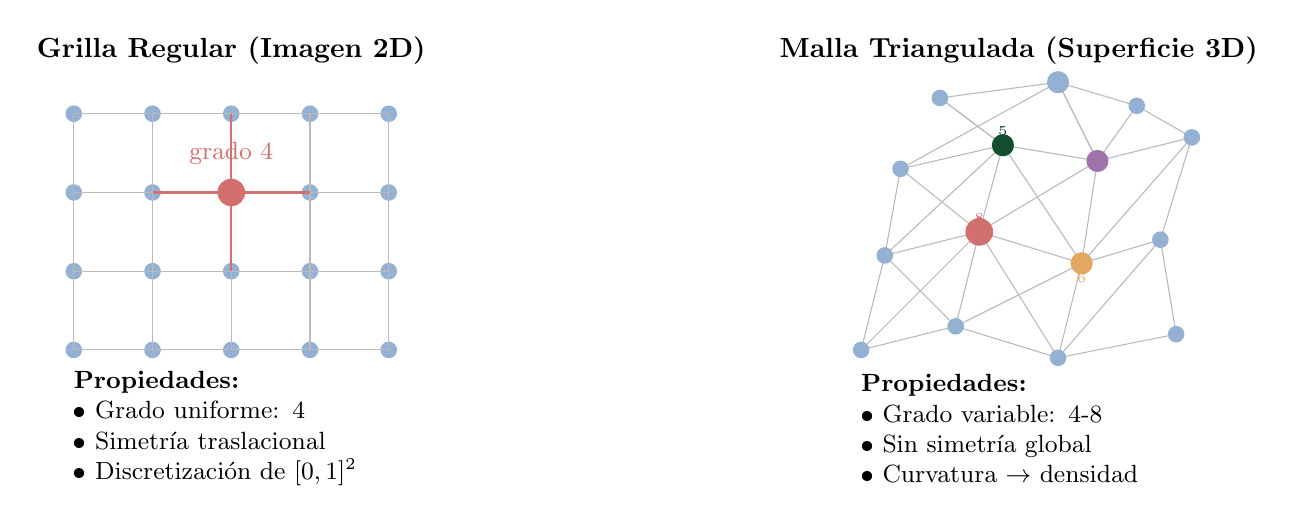
\begin{tikzpicture}

% === Panel izquierdo: Grilla regular ===
\begin{scope}[shift={(-5,0)}]
    \node[above, font=\bfseries] at (2, 3.5) {Grilla Regular (Imagen 2D)};

    % Grid
    \foreach \x in {0,1,2,3,4} {
        \foreach \y in {0,1,2,3} {
            \fill[gdlblue!50] (\x, \y) circle (3pt);
        }
    }

    % Edges horizontales
    \foreach \x in {0,1,2,3} {
        \foreach \y in {0,1,2,3} {
            \draw[gdlgray!60] (\x, \y) -- (\x+1, \y);
        }
    }

    % Edges verticales
    \foreach \x in {0,1,2,3,4} {
        \foreach \y in {0,1,2} {
            \draw[gdlgray!60] (\x, \y) -- (\x, \y+1);
        }
    }

    % Destacar un nodo interior
    \fill[gdlred!70] (2, 2) circle (5pt);
    \draw[thick, gdlred!70] (2,2) -- (1,2);
    \draw[thick, gdlred!70] (2,2) -- (3,2);
    \draw[thick, gdlred!70] (2,2) -- (2,1);
    \draw[thick, gdlred!70] (2,2) -- (2,3);

    % Etiquetas
    \node[font=\small, gdlred!70] at (2, 2.5) {grado 4};

    \node[font=\small, text width=4cm] at (2, -1) {
        \textbf{Propiedades:}\\
        • Grado uniforme: 4\\
        • Simetría traslacional\\
        • Discretización de $[0,1]^2$
    };
\end{scope}

% === Panel derecho: Malla triangulada ===
\begin{scope}[shift={(5,0)}]
    \node[above, font=\bfseries] at (2, 3.5) {Malla Triangulada (Superficie 3D)};

    % Vértices (posiciones irregulares)
    \coordinate (v1) at (0, 0);
    \coordinate (v2) at (1.2, 0.3);
    \coordinate (v3) at (2.5, -0.1);
    \coordinate (v4) at (4, 0.2);
    \coordinate (v5) at (0.3, 1.2);
    \coordinate (v6) at (1.5, 1.5);
    \coordinate (v7) at (2.8, 1.1);
    \coordinate (v8) at (3.8, 1.4);
    \coordinate (v9) at (0.5, 2.3);
    \coordinate (v10) at (1.8, 2.6);
    \coordinate (v11) at (3, 2.4);
    \coordinate (v12) at (4.2, 2.7);
    \coordinate (v13) at (1, 3.2);
    \coordinate (v14) at (2.5, 3.4);
    \coordinate (v15) at (3.5, 3.1);

    % Triangulación (aristas)
    \draw[gdlgray!60] (v1) -- (v2) -- (v3) -- (v4);
    \draw[gdlgray!60] (v5) -- (v6) -- (v7) -- (v8);
    \draw[gdlgray!60] (v9) -- (v10) -- (v11) -- (v12);
    \draw[gdlgray!60] (v13) -- (v14) -- (v15);

    \draw[gdlgray!60] (v1) -- (v5) -- (v9);
    \draw[gdlgray!60] (v2) -- (v6) -- (v10) -- (v13);
    \draw[gdlgray!60] (v3) -- (v7) -- (v11) -- (v14);
    \draw[gdlgray!60] (v4) -- (v8) -- (v12) -- (v15);

    \draw[gdlgray!60] (v1) -- (v6);
    \draw[gdlgray!60] (v2) -- (v5);
    \draw[gdlgray!60] (v2) -- (v7);
    \draw[gdlgray!60] (v3) -- (v6);
    \draw[gdlgray!60] (v3) -- (v8);
    \draw[gdlgray!60] (v5) -- (v10);
    \draw[gdlgray!60] (v6) -- (v9);
    \draw[gdlgray!60] (v6) -- (v11);
    \draw[gdlgray!60] (v7) -- (v10);
    \draw[gdlgray!60] (v7) -- (v12);
    \draw[gdlgray!60] (v9) -- (v14);
    \draw[gdlgray!60] (v10) -- (v13);
    \draw[gdlgray!60] (v11) -- (v14);
    \draw[gdlgray!60] (v11) -- (v15);

    % Vértices
    \foreach \v in {v1,v2,v3,v4,v5,v8,v9,v12,v13,v15} {
        \fill[gdlblue!50] (\v) circle (3pt);
    }

    % Nodos con diferentes grados
    \fill[gdlred!70] (v6) circle (5pt);  % grado alto
    \fill[gdlorange!70] (v7) circle (4pt);  % grado medio
    \fill[gdlgreen!60!black] (v10) circle (4pt);
    \fill[gdlpurple!70] (v11) circle (4pt);
    \fill[gdlblue!50] (v14) circle (4pt);

    % Etiquetas de grado
    \node[font=\tiny, gdlred!70, above] at (v6) {8};
    \node[font=\tiny, gdlorange!70, below] at (v7) {6};
    \node[font=\tiny, gdlgreen!60!black, above] at (v10) {5};

    \node[font=\small, text width=4cm] at (2, -1) {
        \textbf{Propiedades:}\\
        • Grado variable: 4-8\\
        • Sin simetría global\\
        • Curvatura $\to$ densidad
    };
\end{scope}

\end{tikzpicture}
\end{document}
